\session{Lecture 2}{The cosmic microwave background}{II. From primordial fluctuations to real data}

\begin{frame}{Lecture 1 in four steps}
\begin{columns}[T]
\column{.47\textwidth}
\begin{block}{1. Expanding background}
$H^2=(8\pi G/3)\rho$ sets the thermal history and the relation between time and scale factor.
\end{block}
\begin{block}{2. Recombination}
The falling free-electron abundance makes the photon mean free path grow; the visibility $g(\tau)$ locates last scattering.
\end{block}
\column{.47\textwidth}
\begin{block}{3. Fourier modes}
At linear order, each spatial wavevector $\bk$ evolves independently.
\end{block}
\begin{block}{4. Acoustic dynamics}
Photon pressure and baryon inertia drive oscillations in $X\equiv\Theta_0+\Psi$ and the photon--baryon velocity.
\end{block}
\end{columns}
\key{Today we project those three-dimensional perturbations onto the sky and connect them to measured data.}
\end{frame}

\begin{frame}{Outline for Lecture 2}
\begin{enumerate}
\item Motivate the inflationary initial conditions.
\item Describe a random field on the sky.
\item Derive $C_\ell$ from primordial fluctuations and transfer functions.
\item Read cosmological parameters from the spectrum.
\item Follow an observation from detector to bandpowers.
\item Fit the public Planck temperature data.
\item Look ahead to the next generation of CMB measurements.
\end{enumerate}
\key{Theory becomes a prediction for data, with uncertainties and assumptions.}
\end{frame}

\begin{frame}{Why was inflation proposed?}
\begin{columns}[T]
\column{.47\textwidth}
\begin{block}{Background puzzles}
\begin{itemize}
\item Why is spatial curvature so small?
\item Why is the CMB temperature uniform across regions that appear causally disconnected?
\end{itemize}
\end{block}
\column{.47\textwidth}
\begin{block}{Later observational successes}
\begin{itemize}
\item coherent acoustic phases,
\item nearly scale-invariant fluctuations,
\item predominantly adiabatic initial conditions.
\end{itemize}
\end{block}
\end{columns}
\key{Inflation was proposed to solve background problems; detailed CMB measurements later tested its perturbations.}
\end{frame}

\begin{frame}{Flatness is unstable in a decelerating Universe}
Allow spatial curvature in the Friedmann equation and define
\[
H^2=\frac{8\pi G}{3}\rho-\frac{k}{a^2},
\qquad |\Omega_k|\equiv\frac{|k|}{a^2H^2}.
\]
\begin{columns}[T]
\column{.47\textwidth}
\begin{block}{Radiation domination}
$H^2\propto a^{-4}$, so $|\Omega_k|\propto a^2$.
\end{block}
\column{.47\textwidth}
\begin{block}{Matter domination}
$H^2\propto a^{-3}$, so $|\Omega_k|\propto a$.
\end{block}
\end{columns}
In the ordinary hot-Big-Bang history, any initial curvature grows relative to the dominant density.
\key{The small curvature observed today requires an extraordinarily flat early Universe unless the expansion history changes.}
\end{frame}

\begin{frame}{The uniform CMB poses a causal problem}
\begin{columns}[c]
\column{.53\textwidth}
At last scattering,
\[
\chi_*\simeq14\ {\rm Gpc},
\qquad \chi_H(\tau_*)\sim {\cal O}(10^2)\ {\rm Mpc}.
\]
The causal scale subtends roughly a degree, yet the mean temperature agrees across the whole sky to about one part in $10^5$.
\medskip
In a decelerating history, the comoving particle horizon is finite and grows with time.
\column{.43\textwidth}
\begin{tikzpicture}
\node[inner sep=0] (cmbmap) {\includegraphics[width=\linewidth]{planck-2018-cmb-map.jpg}};
\draw[orange,line width=1.2pt] ($(cmbmap.center)+(1.05,.28)$) circle[radius=.12cm];
\draw[orange,thick,->] ($(cmbmap.center)+(1.14,.38)$) -- ($(cmbmap.center)+(1.72,1.05)$);
\node[fill=white,fill opacity=.88,text opacity=1,rounded corners=1pt,
      align=center,font=\scriptsize,text=navy]
      at ($(cmbmap.center)+(.92,1.38)$)
      {$\sim1^\circ$ causal patch\\marker enlarged};
\end{tikzpicture}
\credit{Planck 2018 temperature map.}
\end{columns}
\key{What established almost the same initial state in regions that could not communicate in the standard history?}
\end{frame}

\begin{frame}{Accelerated expansion changes the causal history}
\small
Inflation is accelerated \emph{expansion}:
\[
\dot a>0,\qquad \ddot a>0.
\]
Since $aH=\dot a$, the more general condition is
\[
\frac{d}{dt}\frac{1}{|aH|}<0
\quad\Longleftrightarrow\quad
\dot a\,\ddot a>0.
\]
{\scriptsize The other branch, $\dot a<0$ and $\ddot a<0$, is accelerated contraction rather than inflation.}
\begin{columns}[T]
\column{.47\textwidth}
\begin{block}{Flatness}
$|\Omega_k|\propto(aH)^{-2}\to0$: curvature is dynamically suppressed.
\end{block}
\column{.47\textwidth}
\begin{block}{Causal history}
Our observed region can originate inside one smaller patch with a common causal past.
\end{block}
\end{columns}
\key{The same accelerated expansion addresses both the flatness and horizon problems.}
\end{frame}

\begin{frame}{A mode exits during inflation and re-enters later}
\begin{center}
\includegraphics[width=.82\linewidth,height=5.55cm,keepaspectratio]{inflation-horizon.png}
\end{center}
\credit{The solid horizontal line is one fixed comoving wavelength $k^{-1}$; the dashed line is $(aH)^{-1}$.}
\end{frame}

\begin{frame}{The CMB later tested inflationary perturbations}
\begin{columns}[T]
\column{.47\textwidth}
\begin{block}{Coherent phases}
Sharp acoustic peaks require Fourier modes to enter the horizon with synchronized temporal phases.
\end{block}
\begin{block}{Adiabaticity}
The species begin predominantly in one common, single-clock perturbation.
\end{block}
\column{.47\textwidth}
\begin{block}{Measured near scale invariance}
The inferred primordial power spectrum is
\[
\Delta_{\Rs}^2(k)=A_s\left(\frac{k}{k_0}\right)^{n_s-1},
\qquad n_s\simeq1.
\]
The power per logarithmic interval changes only slowly with scale.
\end{block}
\end{columns}
\key{Inflation supplies a statistical initial field; the later plasma evolution and projection turn it into the observed CMB.}
\end{frame}

\begin{frame}{What reaches us from last scattering?}
\small
We quote the linear line-of-sight result in the instantaneous-recombination approximation:
\[
\Theta(\bn)=\underbrace{[\Theta_0+\Psi]_*}_{\text{intrinsic + gravity}}
-\underbrace{\bn\cdot\bv_b|_*}_{\text{Doppler}}
+\underbrace{\int_{\tau_*}^{\tau_0}(\dot\Phi+\dot\Psi)d\tau}_{\text{integrated gravity}}.
\]
\normalsize
\begin{itemize}
\item Lecture 1 developed the acoustic dynamics controlling $X_* = [\Theta_0+\Psi]_*$ and $\bv_b|_*$.
\item Evolving potentials add an integrated Sachs--Wolfe contribution.
\item Our task now is to project these sources onto the sky and derive $C_\ell$.
\end{itemize}
\credit{We use this source decomposition as our starting point; deriving it requires the photon Boltzmann or geodesic equation. $\bn$ points from us toward the emission position. Observer monopole and dipole terms have been removed; $c=1$.}
\end{frame}

\begin{frame}{One 3D Fourier wave projects onto many angular multipoles}
\begin{columns}[c]
\column{.44\textwidth}
Choose one fixed wavevector $\bk$, with magnitude $k=|\bk|$. On the last-scattering sphere,
\[\bx_* =\chi_*\bn,\qquad e^{i\bk\cdot\bx_*}=e^{ik\chi_*\mu},\]
where $\mu=\hat{\bk}\cdot\bn$. As $\bn$ varies across the sky, this one plane wave produces an angular pattern containing a range of $\ell$ values.
\key{Useful estimate: $\ell\sim k\chi_*$. Projection has finite width.}
\column{.53\textwidth}\includegraphics[width=\linewidth]{bessel-projection.pdf}
\end{columns}
\end{frame}

\begin{frame}{Spherical harmonics are the natural angular basis}
\plot{harmonics.pdf}{These are mathematical basis functions. Increasing $\ell$ resolves finer angular structure; an observed CMB map is a superposition of many such patterns.}
\end{frame}

\begin{frame}{Separate the sky from its statistical description}
\[\Theta(\bn)=\sum_{\ell m}a_{\ell m}Y_{\ell m}(\bn),\qquad
a_{\ell m}=\int d\Omega\,Y^*_{\ell m}\Theta.\]
\begin{itemize}
\item $\ell=0$: monopole; $\ell=1$: dipole.
\item Rough angular feature size: $\pi/\ell$.
\item At each $\ell$, there are $2\ell+1$ values of $m$.
\end{itemize}
\key{The coefficients $a_{\ell m}$ describe our particular realization of the sky.}
\credit{Here $a_{\ell m}$ describes fractional temperature $\Theta$. The mean and motion dipole are normally removed in anisotropy analysis.}
\end{frame}

\begin{frame}{Statistical isotropy defines the power spectrum}
\[\boxed{\langle a_{\ell m}a^*_{\ell'm'}\rangle
=C_\ell\delta_{\ell\ell'}\delta_{mm'}.}\]
\begin{itemize}
\item An ensemble average is over hypothetical skies with the same cosmology.
\item No preferred orientation: every $m$ at fixed $\ell$ has the same variance.
\item For a Gaussian field, mean and covariance specify its statistics.
\end{itemize}
\[\langle\Theta(\bn)\Theta(\bn')\rangle
=\sum_\ell\frac{2\ell+1}{4\pi}C_\ell P_\ell(\bn\cdot\bn').\]
\end{frame}

\begin{frame}{We estimate an ensemble variance from one sky}
For a full, noiseless sky,
\[\widehat C_\ell=\frac1{2\ell+1}\sum_m|a_{\ell m}|^2.\]
For Gaussian perturbations,
\[\boxed{\mathrm{Var}(\widehat C_\ell)=\frac{2}{2\ell+1}C_\ell^2.}\]
\key{Cosmic variance survives even with a perfect instrument.}
\end{frame}

\begin{frame}{The largest angular scales offer the fewest modes}
\plot{cosmic-variance.pdf}{This is usually called \emph{mode counting}: at fixed $\ell$, the sky provides $2\ell+1$ modes. Full sky, Gaussian statistics, no noise or foregrounds.}
\end{frame}

\begin{frame}{Keep track of which spectrum is being plotted}
\[D_\ell=\frac{\ell(\ell+1)}{2\pi}C_\ell.\]
The derivation uses dimensionless $\Theta=\delta T/T_0$.
\[C_\ell^{\delta T\delta T}=T_0^2 C_\ell^{\Theta\Theta}.\]
\begin{itemize}
\item Put $T_0$ in $\mu$K to obtain a spectrum in $\mu$K$^2$.
\item The same conversion applies to $D_\ell$.
\item Observational plots below show $D_\ell^{TT}$ in $\mu$K$^2$.
\end{itemize}
\end{frame}

\begin{frame}{Initial conditions: a random curvature field}
Using the Fourier convention from Lecture 1,
\[\langle\Rs_i(\bk)\Rs_i^*(\bk')\rangle
=(2\pi)^3\delta^{(3)}(\bk-\bk')P_{\Rs}(k),\]
\[P_{\Rs}(k)=\frac{2\pi^2}{k^3}\Delta_{\Rs}^2(k),\qquad
\Delta_{\Rs}^2(k)=A_s\left(\frac{k}{k_0}\right)^{n_s-1}.\]
\key{Random initial amplitudes; deterministic linear evolution for each mode.}
\credit{Equivalently, without complex conjugation the delta function is $\delta^{(3)}(\bk+\bk')$, as in the notes.}
\end{frame}

\begin{frame}{Projection step 1: expand a plane wave}
\[e^{ix\mu}=\sum_\ell i^\ell(2\ell+1)j_\ell(x)P_\ell(\mu).\]
Evolution and projection together define the transfer function:
\small
\[\Theta(\bn)=\sum_\ell i^\ell(2\ell+1)
\int\frac{d^3k}{(2\pi)^3}\Rs_i(\bk)\Theta_\ell(k)
P_\ell(\hat{\bk}\cdot\bn).\]
\normalsize
\key{$\Theta_\ell(k)$ is the temperature response per unit initial curvature perturbation.}
\end{frame}

\begin{frame}{Projection step 2: identify the harmonic coefficients}
The addition theorem is
\[P_\ell(\hat{\bk}\cdot\bn)=\frac{4\pi}{2\ell+1}
\sum_mY^*_{\ell m}(\hat{\bk})Y_{\ell m}(\bn).\]
Insert it in the plane-wave expansion and compare coefficients:
\[\boxed{a_{\ell m}=4\pi i^\ell\int\frac{d^3k}{(2\pi)^3}
\Rs_i(\bk)\Theta_\ell(k)Y^*_{\ell m}(\hat{\bk}).}\]
\end{frame}

\begin{frame}{Use the primordial statistics to obtain $C_\ell$}
\small
\[
\begin{aligned}
\langle a_{\ell m}a^*_{\ell'm'}\rangle
={}&(4\pi)^2i^{\ell-\ell'}
\int\frac{d^3k}{(2\pi)^3}P_{\Rs}(k)\\
&\times\Theta_\ell(k)\Theta_{\ell'}(k)
Y^*_{\ell m}(\hat{\bk})Y_{\ell'm'}(\hat{\bk}).
\end{aligned}
\]
\normalsize
\begin{enumerate}
\item The primordial delta function removes one momentum integral.
\item Harmonic orthogonality gives $\delta_{\ell\ell'}\delta_{mm'}$.
\item $d^3k=k^2dk\,d\Omega_k$ leaves a radial integral.
\end{enumerate}
\[\frac{(4\pi)^2}{(2\pi)^3}\,k^2dk\,\frac{2\pi^2}{k^3}
=4\pi\,d\ln k.\]
\end{frame}

\begin{frame}{Primordial power and transfer functions determine $C_\ell$}
\[\boxed{C_\ell^{\Theta\Theta}=4\pi\int d\ln k\,
\Delta_{\Rs}^2(k)\Theta_\ell^2(k).}\]
\begin{columns}[T]
\column{.47\textwidth}
\begin{block}{Primordial input}
$\Delta_{\Rs}^2(k)$\par\medskip
Amplitude, tilt, and possible features in the initial curvature spectrum.
\end{block}
\column{.47\textwidth}
\begin{block}{Evolution and projection}
$\Theta_\ell(k)$\par\medskip
Gravity, acoustics, recombination, diffusion, and geometry.
\end{block}
\end{columns}
\credit{The formula is dimensionless here. Multiply by $T_0^2$ for temperature units.}
\end{frame}

\begin{frame}{Check the result on large scales}
In the matter-era Sachs--Wolfe approximation,
\[\Theta_\ell(k)\simeq\frac15j_\ell(k\chi_*).\]
For $\Delta_{\Rs}^2=A_s$ and $\ell\geq1$,
\[\int_0^\infty\frac{dk}{k}j_\ell^2(k\chi_*)
=\frac1{2\ell(\ell+1)}.\]
\[\boxed{D_\ell^{\Theta\Theta}\simeq\frac{A_s}{25}.}\]
\credit{The plateau is an approximation: late-time ISW and other effects alter the largest scales.}
\end{frame}

\begin{frame}{From the sky signal to the source function}
\small
Let $\chi(\tau)=\tau_0-\tau$ and $g=-\dot{\widetilde\tau}e^{-\widetilde\tau}$ be the visibility. Projecting the three terms from slide 3 gives, schematically,
\[
\Theta_\ell(k)\simeq\int_0^{\tau_0}\!d\tau\,
\bigl[
\underbrace{gX\,j_\ell(k\chi)}_{\text{intrinsic + gravity}}
+\underbrace{g v_b\,j_\ell'(k\chi)}_{\text{Doppler}}
+\underbrace{e^{-\widetilde\tau}(\dot\Phi+\dot\Psi)j_\ell(k\chi)}_{\text{integrated gravity}}
+\cdots\bigr].
\]
Integrating the Doppler term by parts moves the derivative from $j_\ell$ into its coefficient. All coefficients of $j_\ell$ can then be collected into one function:
\[
\boxed{\Theta_\ell(k)=\int_0^{\tau_0}d\tau\,S_T(k,\tau)
j_\ell[k(\tau_0-\tau)].}
\]
\key{$S_T$ packages the emission, Doppler, and integrated-gravity sources already introduced on slide 3.}
\credit{The ellipsis includes polarization and other exact linear terms. Signs and velocity factors depend on Fourier conventions. CAMB and CLASS evaluate the complete expression.}
\end{frame}

\begin{frame}{Six parameters; many coupled signatures}
\[\{\omega_b,\omega_c,\theta_s,\tau_{\rm reio},A_s,n_s\},
\qquad \omega_i=\Omega_i h^2.\]
\begin{itemize}
\item Positions: sound horizon divided by distance.
\item Heights: baryon loading, gravitational driving, primordial amplitude.
\item Envelope: primordial tilt, diffusion, reionization, and lensing.
\end{itemize}
\key{No cosmological parameter changes only one feature.}
\credit{Next figures: CAMB lensed spectra. One input is changed at a time while the remaining inputs are held fixed. The curves illustrate physical responses; no data are fitted.}
\end{frame}

\begin{frame}{Increase the baryon density}
\plot{parameter-baryons.pdf}{Change $\omega_b$ at fixed $H_0$, $\omega_c$, and primordial/reionization inputs. Compression versus rarefaction changes, but so do sound speed, diffusion, and distances.}
\end{frame}

\begin{frame}{Increase the cold-dark-matter density}
\plot{parameter-matter.pdf}{Larger $\omega_c$ moves equality earlier and changes potential decay and radiation driving. The other input parameters are fixed, while derived scales respond consistently.}
\end{frame}

\begin{frame}{Change the geometry between us and last scattering}
\plot{parameter-geometry.pdf}{Vary $H_0$ in flat $\Lambda$CDM at fixed physical matter densities. The derived $\Omega_i$ and distances change, so the response includes more than a horizontal rescaling.}
\end{frame}

\begin{frame}{Increase the primordial amplitude}
\plot{parameter-amplitude.pdf}{Larger $A_s$ raises primary power. These spectra include lensing, which also responds to the change.}
\end{frame}

\begin{frame}{Change the primordial tilt}
\plot{parameter-tilt.pdf}{Change $n_s$ at fixed $A_s$ at pivot $k_0=0.05\,\mathrm{Mpc}^{-1}$. Small-scale and large-scale power respond differently.}
\end{frame}

\begin{frame}{Reionization suppresses small scales and creates large-scale polarization}
\plot{parameter-reionization.pdf}{Fixed $A_s$: primary small-scale power is suppressed approximately by $e^{-2\tau_{\rm reio}}$, while large-scale EE gains a reionization feature.}
\end{frame}

\begin{frame}{Polarization gives another view of the acoustic phase}
\plot{polarization.pdf}{Fiducial CAMB spectra. Thomson scattering of a quadrupole generates polarization. EE peaks and TE sign changes test the relative phases of the sources.}
\end{frame}

\begin{frame}{Lensing and parameter degeneracies affect the spectrum}
\[X(\bn)\longrightarrow X(\bn+\nabla\phi).\]
\begin{itemize}
\item Lensing smooths acoustic peaks and converts E into B.
\item Its induced four-point correlations let us reconstruct $\phi$.
\item High-$\ell$ primary amplitudes mainly measure $A_se^{-2\tau_{\rm reio}}$.
\item Different expansion histories can preserve $r_s/\chi_*$.
\end{itemize}
\end{frame}

\begin{frame}{Ten-minute break}
\vfill\Large We can now predict $C_\ell$ and understand how its features respond to cosmological parameters.
\medskip\par Next: how an experiment turns detector samples into bandpowers and parameter constraints.
\vfill
\end{frame}

\begin{frame}{How does an experiment produce these points?}
\begin{center}
\begin{tikzpicture}[node distance=6mm and 9mm,
box/.style={draw=teal,fill=pale,rounded corners,minimum width=33mm,minimum height=12mm,align=center},
arr/.style={-{Stealth},thick,navy}]
\node[box] (d) {detector\\timestreams};
\node[box,right=of d] (m) {frequency\\maps};
\node[box,right=of m] (f) {foreground\\treatment};
\node[box,below=of f] (b) {spectra /\\bandpowers};
\node[box,left=of b] (l) {likelihood +\\nuisance model};
\node[box,left=of l] (p) {cosmological\\posterior};
\draw[arr] (d)--(m);\draw[arr] (m)--(f);\draw[arr] (f)--(b);
\draw[arr] (b)--(l);\draw[arr] (l)--(p);
\end{tikzpicture}
\end{center}
\key{A published spectrum is already the result of several inference steps.}
\end{frame}

\begin{frame}{The measurement begins with detector time streams}
\[d_t=g_t[I_p+Q_p\cos2\gamma_t+U_p\sin2\gamma_t]+n_t+s_t.\]
\begin{itemize}
\item $d_t$ is one detector sample at time index $t$; pointing selects $p=p(t)$ and $\gamma_t$ is the detector orientation.
\item $I$ is total intensity; $Q$ and $U$ describe linear polarization in a chosen pair of sky axes.
\item Calibration $g_t$, beam, bandpass, and detector response matter.
\item Noise $n_t$ can be correlated in time; $s_t$ represents systematics.
\end{itemize}
\end{frame}

\begin{frame}{Map-making combines repeated observations}
\[\mathbf d=\mathbf A\mathbf m+\mathbf n.\]
Here $\mathbf d=(d_1,\ldots,d_{N_t})^T$ is the full data vector and $\mathbf m$ stacks the map values $(I_p,Q_p,U_p)$.
For Gaussian noise covariance $\mathbf N$,
\[\widehat{\mathbf m}=(\mathbf A^T\mathbf N^{-1}\mathbf A)^{-1}
\mathbf A^T\mathbf N^{-1}\mathbf d.\]
\begin{itemize}
\item $\mathbf A$ encodes pointing and polarization orientation.
\item Repeated scans constrain the same sky pixels.
\item Data splits and difference maps test residual systematics.
\end{itemize}
\credit{This is the idealized linear map-making problem; practical analyses also model calibration, filtering, and other effects.}
\end{frame}

\begin{frame}{Frequency information separates sky components}
\[m_\nu(\bn)=a_{\rm CMB}(\bn)+\sum_c f_\nu^c(\bm\beta_c,\bn)a_c(\bn)+n_\nu.\]
\begin{itemize}
\item In thermodynamic-temperature units, the CMB response is frequency independent.
\item Galactic synchrotron and dust have different spectra.
\item Temperature also contains compact sources and extragalactic signals.
\end{itemize}
\key{Foreground treatment can happen in maps, in spectra, or jointly in a likelihood. Its uncertainty must propagate.}
\end{frame}

\begin{frame}{Masks and beams change the spectrum you measure}
\[\langle\widetilde C_\ell\rangle
=\sum_{\ell'}M_{\ell\ell'}B_{\ell'}^2F_{\ell'}C_{\ell'}+\widetilde N_\ell.\]
\begin{itemize}
\item Mask coupling $M$: partial sky mixes harmonic modes.
\item Beam $B_\ell$: finite resolution suppresses small scales.
\item Filtering $F_\ell$: processing can remove or attenuate modes.
\item Noise adds power to an auto-spectrum.
\end{itemize}
\credit{Bandpowers group nearby multipoles; windows and covariances specify how to compare them with theory.}
\end{frame}

\begin{frame}{Cross-spectra remove independent noise bias}
For two maps with common sky and independent zero-mean noise,
\[\langle(s+n_1)(s+n_2)^*\rangle=\langle|s|^2\rangle.\]
There is no mean independent-noise bias, but there is still noise variance.
\[\mathrm{Var}(\widehat C_\ell)\approx
\frac{2}{(2\ell+1)f_{\rm sky}}(C_\ell+N_\ell)^2.\]
\credit{The last expression is an approximate auto-spectrum uncertainty estimate. Real cross-spectrum and bandpower covariances require their own noise and coupling terms.}
\end{frame}

\begin{frame}{The likelihood includes cosmology and nuisance parameters}
\small
\[P(\bm\theta,\bm\eta\mid\mathbf d)\propto
\mathcal L[\mathbf d\mid C_\ell(\bm\theta),\bm\eta]
P(\bm\theta)P(\bm\eta).\]
\normalsize
\begin{itemize}
\item $\bm\theta$: cosmological parameters; $\bm\eta$: nuisance parameters.
\item An Einstein--Boltzmann solver predicts the spectra.
\item Covariances, foregrounds, calibration, and priors enter the comparison.
\end{itemize}
\key{Our classroom fit will isolate two ideas inside this larger calculation.}
\end{frame}

\begin{frame}{Now work with real Planck data}
\Large\colabtwo\normalsize
\medskip\par The public table contains
\[\{\ell_{\rm eff},D_b^{\rm data},\sigma_-,\sigma_+,D_b^{\rm template}\}.\]
\begin{enumerate}
\item Plot the bandpowers and the published best-fit template.
\item Fit an amplitude and an angular dilation.
\item Inspect residuals and parameter correlations.
\end{enumerate}
\credit{Planck 2018 PR3 binned TT spectrum, distributed via the NASA/IPAC mirror. Embedded results provide an offline fallback.}
\end{frame}

\begin{frame}{Two parameters isolate two observable effects}
\[\boxed{D_\ell^{\rm model}(A,\alpha)=A\,D_{\alpha\ell}^{\rm template}.}\]
\begin{itemize}
\item $A$ changes the vertical amplitude.
\item $\alpha$ dilates the multipole argument.
\item A template peak at $\ell_p$ appears at $\ell_p/\alpha$.
\end{itemize}
\credit{$A$ and $\alpha$ are phenomenological template parameters. Mapping them onto $A_s$, $H_0$, or $\theta_s$ requires a physical cosmological model.}
\end{frame}

\begin{frame}{A simple likelihood for the Planck exercise}
\[\sigma_b=\frac{\sigma_{b,-}+\sigma_{b,+}}2,\qquad
\chi^2(A,\alpha)=\sum_b\frac{[D_b^{\rm data}-D_b^{\rm model}]^2}{\sigma_b^2}.\]
\begin{itemize}
\item Use $50<\ell<2000$.
\item Interpolate the supplied template; approximate bandpower errors as independent Gaussian errors.
\item Find the minimum and inspect the residuals.
\end{itemize}
\key{These assumptions make the calculation transparent. The official Planck analysis uses a fuller data and covariance model.}
\end{frame}

\begin{frame}{A fit must explain the residuals as well as the curve}
\plot{planck-notebook-2.png}{Actual executed notebook result. Pull $=(D_b^{\rm data}-D_b^{\rm model})/\sigma_b$. Examine patterns, outliers, and the role of the fitting range.}
\end{frame}

\begin{frame}{The fit has correlated uncertainties}
\begin{columns}[c]
\column{.56\textwidth}\includegraphics[width=\linewidth,height=5.3cm,keepaspectratio]{planck-notebook-3.png}
\column{.41\textwidth}
\small
Executed teaching fit:
\[A=1.00011\pm0.00137\]
\[\alpha=1.000026\pm0.000382\]
\[\chi^2/\mathrm{dof}=58.7/63\]
Errors use the local curvature approximation.
\medskip\par Contours show approximately 68\% and 95\% for two parameters under the simplified likelihood.
\end{columns}
\credit{These errors are conditional on the supplied template and simplified covariance. Cosmological-parameter uncertainties require a physical model and the full likelihood.}
\end{frame}

\begin{frame}{What did the exercise actually measure?}
\begin{itemize}
\item It compares data with a two-parameter deformation of a fitted template.
\item The template already comes from fitting essentially these data: $A\simeq\alpha\simeq1$ is expected.
\item Correlated errors, foreground/calibration nuisance terms, and low-$\ell$ likelihood structure are simplified or omitted.
\end{itemize}
\key{A small statistical error can depend strongly on the model and what was held fixed.}
\end{frame}

\begin{frame}{What limits the next CMB measurement?}
For a measured sky fraction $f_{\rm sky}$, a useful approximation is
\[
\sigma(\widehat C_\ell)\simeq
\sqrt{\frac{2}{(2\ell+1)f_{\rm sky}}}\,(C_\ell+N_\ell).
\]
\begin{columns}[T]
\column{.31\textwidth}
\begin{block}{Instrument}
Lower $N_\ell$ with more sensitivity, better resolution, and controlled systematics.
\end{block}
\column{.31\textwidth}
\begin{block}{Modes}
Increase sky area and the range of angular scales that carry useful signal.
\end{block}
\column{.31\textwidth}
\begin{block}{Sky emission}
Use frequency information to separate the CMB from foregrounds.
\end{block}
\end{columns}
\key{Future surveys improve constraints by making more independent modes usable.}
\end{frame}

\begin{frame}{CMB sensitivity has followed a Moore's-law trend}
\begin{center}
\includegraphics[width=.75\linewidth,height=5.15cm,keepaspectratio]{cmb-detector-moore-law.png}
\end{center}
\credit{Historical sensitivity trend and stage definitions from the CMB-S4 Science Book, Fig.~2 (arXiv:1610.02743). The dashed curves were projections, not a present-day project schedule. The quoted trend corresponds to a sensitivity doubling roughly every 2.3 years.}
\end{frame}

\begin{frame}{Background-limited detectors make large arrays essential}
\begin{itemize}
\item Modern CMB bolometers can approach the photon-noise floor set by the sky, atmosphere, and telescope.
\item It contains Poisson fluctuations in photon counts and correlations between thermal-photon arrivals (``wave'' or ``bunching'' noise).
\end{itemize}
For approximately independent detectors,
\[
\boxed{\mathrm{NET}_{\rm array}\simeq
\frac{\mathrm{NET}_{\rm det}}{\sqrt{N_{\rm det}}}},
\qquad
\boxed{\text{mapping speed}\propto N_{\rm det}}.
\]
\key{The practical route to deeper maps is to observe with more background-limited detectors for longer.}
\credit{Detector yield, correlated noise, readout, calibration, and observing efficiency limit this ideal scaling.}
\end{frame}

\begin{frame}{More sensitivity gives access to more modes}
The number of full-sky harmonic modes up to $\ell_{\max}$ is
\[
N_{\rm modes}=f_{\rm sky}\sum_{\ell=2}^{\ell_{\max}}(2\ell+1)
\simeq f_{\rm sky}\ell_{\max}^2.
\]
\begin{itemize}
\item Lower noise makes polarization and smaller-scale modes measurable.
\item Larger sky coverage raises $f_{\rm sky}$ and supplies more independent modes.
\item When $N_\ell\ll C_\ell$, the same sky is cosmic-variance limited; additional detectors bring little improvement for that spectrum.
\end{itemize}
\key{This is mode counting again: parameter errors shrink because the data contain more independent measurements.}
\end{frame}

\begin{frame}{Frequency coverage determines which modes remain usable}
\small
\[m_\nu(\bn)=a_{\rm CMB}(\bn)
+f_\nu^{\rm sync}a_{\rm sync}(\bn)
+f_\nu^{\rm dust}a_{\rm dust}(\bn)+\cdots\]
\normalsize
\begin{center}
\begin{tikzpicture}[x=1cm,y=1cm]
\draw[-{Stealth},thick,navy] (0,0)--(11,0) node[right]{frequency};
\foreach \x/\lab in {0.6/30,4.0/100,7.4/300,10.8/1000}
  {\draw (\x,.08)--(\x,-.08) node[below]{\lab\,GHz};}
\draw[very thick,orange] (.45,1.55)--(7.05,1.55);
\node[anchor=east] at (.25,1.55){SO};
\node[anchor=west,navy] at (7.15,1.55){27--280 GHz};
\draw[very thick,teal] (.75,1.0)--(8.45,1.0);
\node[anchor=east] at (.25,1.0){LiteBIRD};
\node[anchor=west,navy] at (8.55,1.0){34--448 GHz};
\draw[very thick,navy] (6.55,.45)--(10.35,.45);
\node[anchor=east] at (6.35,.45){CCAT};
\node[anchor=west,navy] at (10.45,.45){220--850 GHz};
\node[teal,anchor=west] at (.2,-.75){synchrotron};
\node[navy] at (5.2,-.75){CMB-dominated bands};
\node[orange,anchor=east] at (10.8,-.75){dust / CIB};
\end{tikzpicture}
\end{center}
\key{Frequency channels do not add copies of the same CMB mode; they let us identify and remove emission with a different spectrum.}
\credit{Band ranges are schematic summaries of the experiment designs. Foreground spectra vary across the sky, so component separation requires more than fitting one universal frequency law.}
\end{frame}

\begin{frame}{Simons Observatory combines large and small apertures}
\begin{center}
\includegraphics[width=.91\linewidth,height=4.65cm,keepaspectratio]{simons-observatory-site.jpg}
\end{center}
\begin{itemize}
\item The 6-m LAT targets arcminute scales; the SATs target degree-scale polarization.
\item The expanded programme adds two SO:UK mid-frequency SATs and a sixth, low-frequency SAT supported through SO:JP.
\end{itemize}
\credit{Official Simons Observatory homepage poster frame. Cerro Toco, Atacama Desert, Chile.}
\end{frame}

\begin{frame}{The expanded SAT array sharpens the inflation test}
\begin{center}
\includegraphics[width=.72\linewidth,height=5.9cm,keepaspectratio]{so-expanded-sat-r-ns.png}
\end{center}
\credit{Red: nominal SO; purple/yellow: full SO optimistic/pessimistic; black: $R^2$ inflation. SO Collaboration, arXiv:2512.15833, Fig.~4; 70\% delensing.}
\end{frame}

\begin{frame}{CCAT extends the view to submillimetre frequencies}
\begin{center}
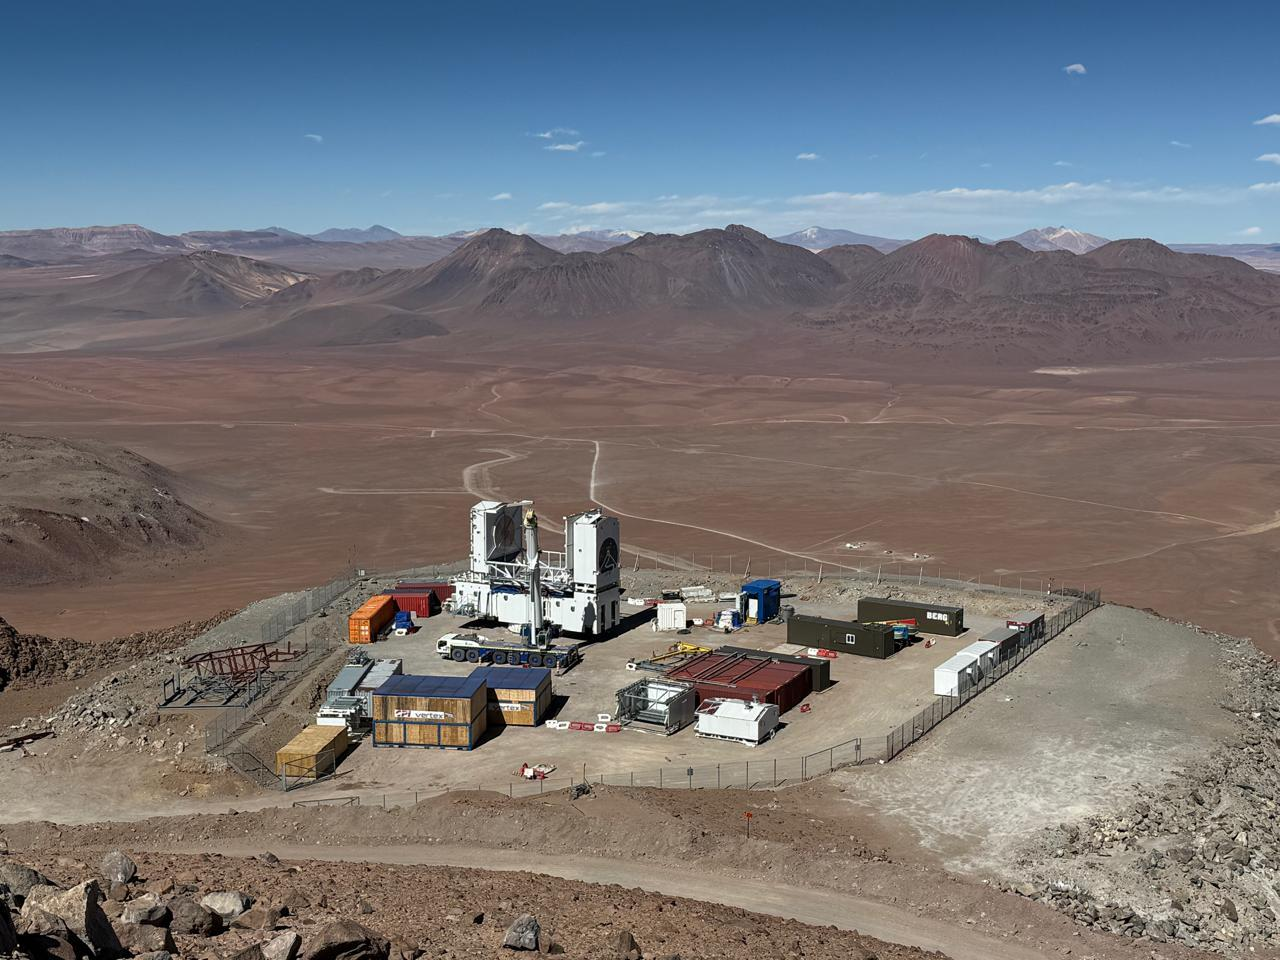
\includegraphics[width=.94\linewidth,height=5.15cm,trim=0 145 0 145,clip]{CCAT-2025-11-17.jpg}
\end{center}
\small Prime-Cam's 220--850 GHz coverage maps dust and the CIB while probing SZ signals, dusty galaxies, and line emission.
\credit{CCAT/Fred Young Submillimeter Telescope. Prime-Cam capabilities: CCAT Observatory science forecasts.}
\end{frame}

\begin{frame}{LiteBIRD targets the largest polarization scales}
\begin{center}
\includegraphics[width=.82\linewidth,height=5.8cm,keepaspectratio,trim=25 0 25 150,clip]{litebird-forecast.png}
\end{center}
\credit{LiteBIRD Collaboration, arXiv:2202.02773, Fig.~1. Mission requirement: total $\delta r<10^{-3}$.}
\end{frame}

\begin{frame}{The CMB is a backlight for the later Universe}
\begin{center}
\includegraphics[width=.99\linewidth,height=5.95cm,keepaspectratio]{cmb-backlight-main.png}
\end{center}
\credit{Colin Hill; based on SO Collaboration, JCAP 2019. Intervening matter lenses, scatters, and frequency-shifts the CMB.}
\end{frame}

\begin{frame}{Higher-order correlations contain additional information}
For a Gaussian sky, the two-point function contains all statistical information. Non-Gaussianity appears in connected higher-order correlations, beginning with the bispectrum:
\[
\langle a_{\ell_1m_1}a_{\ell_2m_2}a_{\ell_3m_3}\rangle_c
=\mathcal G^{m_1m_2m_3}_{\ell_1\ell_2\ell_3}
b_{\ell_1\ell_2\ell_3}.
\]
\begin{columns}[T]
\column{.47\textwidth}
\begin{block}{Primordial}
Interactions and additional fields during inflation can produce non-Gaussian initial conditions.
\end{block}
\column{.47\textwidth}
\begin{block}{Secondary}
Lensing, SZ signals, galaxies, and foregrounds generate non-Gaussianity after recombination.
\end{block}
\end{columns}
\key{Primordial non-Gaussianity is my main research area; secondary signals are both contaminants and valuable probes of structure.}
\end{frame}

\begin{frame}{Galaxy cross-correlations reveal secondary non-Gaussianity}
\begin{center}
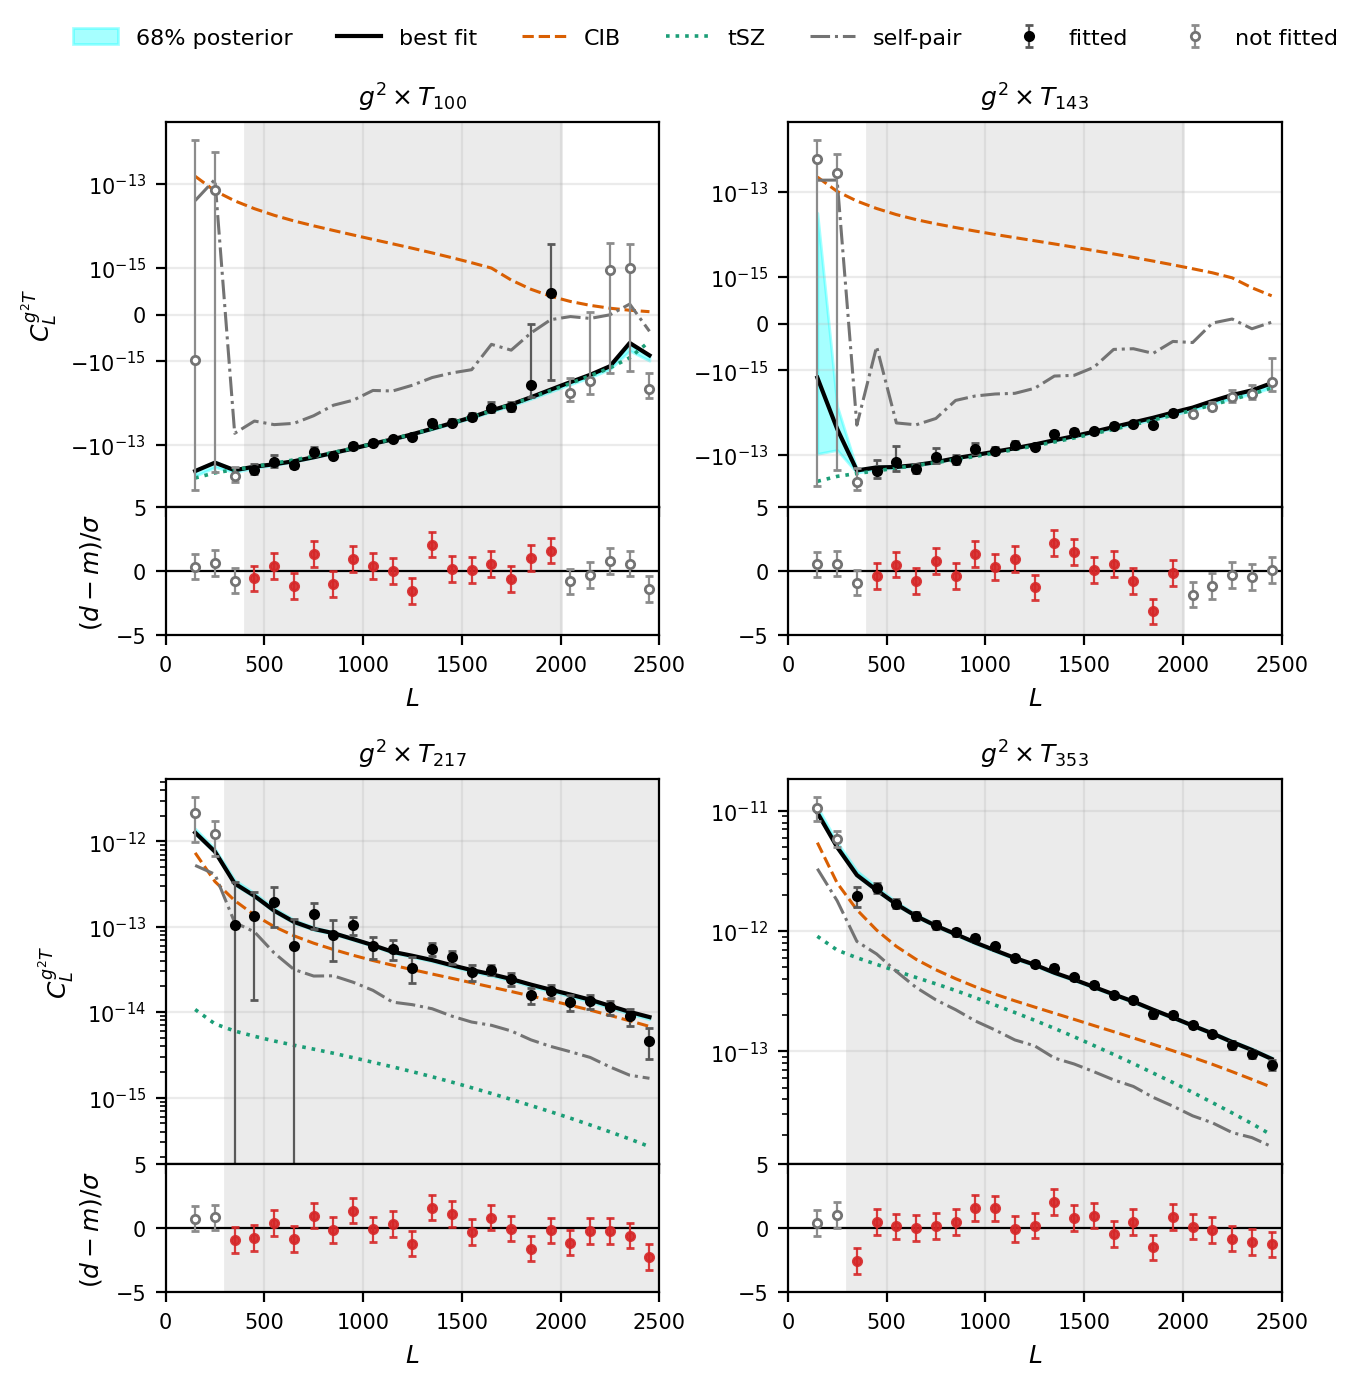
\includegraphics[height=5.75cm,trim=10 10 10 15,clip]{g2t_fit_observed_g2_prl_sellentin_observed_g2_rsz_mmax16_20260925.png}
\end{center}
\credit{$C_L^{g^2T_\nu}$ compresses a galaxy--galaxy--temperature bispectrum. Frequency dependence separates tSZ, CIB, and self-pair terms.}
\end{frame}

\begin{frame}{The full chain}
\begin{columns}[c]
\column{.73\textwidth}
\[\text{primordial fluctuations}\ \longrightarrow\ \text{fluid dynamics}\]
\[\longrightarrow\ \text{projection}\ \longrightarrow\ C_\ell
\ \longrightarrow\ \text{data likelihood}.\]
\key{$\displaystyle C_\ell=4\pi\int d\ln k\,\Delta_{\Rs}^2(k)\Theta_\ell^2(k)$ connects the early Universe to a measurable angular pattern.}
\medskip\par Notes, both notebooks, and executed outputs:
\href{https://github.com/daanmeerburg/RTG_3186_CMB_Lectures}{github.com/daanmeerburg/RTG\_3186\_CMB\_Lectures}
\column{.23\textwidth}
\centering
\qrcode[height=2.45cm]{https://github.com/daanmeerburg/RTG_3186_CMB_Lectures}
\par\smallskip\scriptsize Scan for the public materials.
\end{columns}
\end{frame}
